\documentclass{article}
\usepackage{amsmath,mathtools}
\usepackage{amssymb}
\usepackage{graphicx}
\usepackage{algorithm}
\usepackage{algorithmicx}
\usepackage[noend]{algpseudocode}
\usepackage{algpseudocode}
\usepackage{multicol}
\usepackage{color}
\definecolor{lightyellow}{RGB}{255,255,160}
\usepackage{subcaption}
\DeclareMathOperator*{\argmax}{arg\,max}

\title{Co-Means, Clustering both in visual and histogram space}
\author{}
\date{\today}
\begin{document}
\maketitle

\section{Introduction}
Many denoising methods use image patches comparison, either for point operation[BM3D], or finding nearest neighbors patches in the image, for clusters operation [Non Local means ].

We are looking for a better way of choosing those patches that indeed came from similar Distributions [natural Image Models] and form a cluster from them.

In order to cluster the data, we want to find a way to estimate $ \Pr\{P_{(i)}\in cluster J \}$, and decide a herd assignment function $ \hat{L} $, that maps each pixel in the image to his cluster label:
\begin{equation}
\hat L :(1,..,n)\rightarrow (1,..,K)
\end{equation}

We introduce 'Co-Means' clustering which is based on "centers" in two image features spaces simultaneously.


\section{Motivation}
Clusters based De-noising methods are based on the correctness of the Labeling.
We can think of this clustering given to us by some Oracle to a zero noise image as ground truth. that is we can measure the accuracy of a certain labeling in reference to Oracle Labeling.

Ways to calculate distances between labeling:
\begin{enumerate}
	\item $ \sum_{i=1}^{n} [Oracle_{(i)}\ne\hat{L}_{(i)})]$  - the distance is the amount of mis-labeling
	\item $ \sum_{i=1}^{n} D_K(Oracle_{(i)};\hat{L}_{(i)}) $ where $ D_K(M;L) $ is the distance between label M in the Oracle and Label L in $ \hat{L} $
\end{enumerate}

In the case of noisy image, the clustering problem becomes harder(some problems include over-fitting the noise, loss of relevant structure information...[Irani]). In the noisy case, although each cluster contians noisy data points, the best denoised image, in MSE sense is achieved by using the Oracle labeling. That is because we assume a zero mean noise, and the center of the cluster should still be accurate.
Our goal is to create a labeling method for noisy images that will converge to the Oracle, we describe a way of convergence based on statistics of the labeled image.

\section{Background}
Given an image I with n pixels. We will use, $\hat L$ :(1,..,n)$\rightarrow$ (1,..,K) , assignment function from pixel i$\in(1..n)$ to label J$\in(1..K)$\\
We will use two image features spaces:

\subsection{Visual space}
The feature representing pixel i in visual space will be column stacking of the window patch of size $W_1\times W_1$ around it.
\begin{align*}
& W_{(i)}= I(_{i-\frac{W_1-1}{2}:i+\frac{W_1-1}{2},i-\frac{W_1-1}{2}:i+\frac{W_1-1}{2}}) \\
 &W_{(i)}\in \mathbb{R}^{W_{1}^{2}}
\end{align*}
Center J in visual space will be:  $C_{(J)}=\dfrac{1}{|J|} \Sigma_{\hat{L} (i)=J}P_{(i)}$ i.e., the center of cluster J is the mean of all pixels that are in the cluster ($i\in$ cluster J)\footnote{we use small letters to denote a pixel and Large letters for cluster labels}.

We will denote:
\begin{equation}
\color{red}
P_{i}(J) =\dfrac{1}{Z}exp^{(\dfrac{-dist(P_{(i)} ),C_J)}{\sigma_s〗^2})}〗\label{eq:pixelPr}
\end{equation} 
The probability that pixel i$\in cluster J$,
where $ dist(\cdot,\cdot) $ is the Euclidean distance.(sometimes we will refer as P[i,J] or $ \Pr\{i,J\} $ for matrix notation)

\subsection{Labels histogram space}
For this space, first we will look at an Image that instead of intensity, each pixel value is its cluster label, given by $\hat L$\footnote{Labels is categorical data with no respect to size $ J>K $}.

Each pixel will then be characterized by its label values histogram in a $W_2\times W_2$ surrounding around it (not containing the center pixel).\\
e.g. 
\begin{multicols}{3}
\begin{tabular}{|c|c|c|}\hline
1&5&1\\	\hline
5&\colorbox{yellow}{3}&5\\ \hline
9&8&9\\ \hline
\end{tabular}

\begin{flushright}
	H*[i]=
\end{flushright}	
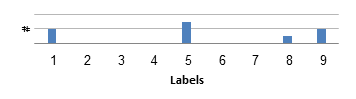
\includegraphics[width=0.9\linewidth]{histogram.png}
\end{multicols}
We denote $ H_{(i)} $ for the Histogram of pixel i in labels space, $ H_{(i)} $  is normalized to 1 (s.t. in the example $ H_{(i)} = \dfrac{\text{H*[i]}}{8}$ )\footnote{generally $\dfrac{\text{H*[i]}}{W_2^2-1}$ }\\
We will also use  $ H_{(i)}(J) $- the J coordinate in $ H_{(i)} $.
\begin{equation*}
\color{red} H_{(i)}\in \mathbb{Z}^K 
\end{equation*}
\subsection{Co-Occurrence}
We use the labels statistics to compute the conditional probability.
$$ \color{red}
 P(K|J)=P _j(K) \ \ s.t. \begin{cases}
&j \in {\mathcal{N}(i)}\\
&\hat{L}(i)=J
\end{cases}  $$
where $ \mathcal{N}(i) $ is the neighbors of pixel i in $ W_2 $ window.
In words we can say this is the probability to witness label K in $ W_2 $ window around a know pixel labeled J.

We arrange $ P(K|J) $ to form a Co-Occurrence matrix, such that each row in the matrix represent $ P(K|J) $

\begin{align}
&CC_J= P(K|J)\label{eq:CoOc}\\
&CC_J=\dfrac{1}{|J|} \sum_{\hat{L}(i)=J}H_{(i)}\nonumber
\end{align}
we denote $ |J|=|\{pixel\ i\in cluster\ J\}| $- the size of cluster J

The Co-Occurrence matrix is not symmetric but can be normalized easily by choosing to use joint probability 
\begin{align}
\color{red}
P(K;J)&=P(K|J)\cdot P(J) \label{eq:jointprob}\\
&where\nonumber\\
P(J)&=\dfrac{\vert J\vert}{n} \nonumber
\end{align}


we surmise that the labels Co-Occurrence matrix should be sparse, that is min $||CoOc||_0$. based on that assumption we will calculate an integrated probability function $\Pr \{P_{(i)}\in cluster J\}$ and show that this regularization derives better assignment. (\colorbox{lightyellow}{unproved yet})


\section{Objective Function}
We would like to update equation \eqref{eq:pixelPr} $ P_{i}(J) $ to relate to a data term $ dist(P_{(i)} ),C_J) $ and regularization in the label space.
We would like to converge to the Oracle CC (which we suppose to be sparse) and not directly to the unknown Oracle.

\subsection{Joint Probability- Message Passing}
We can think on message passing from all of $\mathcal{N}(i)$ neighbors of pixel i, each neighbor thinks its surrounding should be like his Co-Oc.
\begin{equation}
\color{red}
\widetilde{P}_i(K) \leftarrow P_i(K) + \sum_{j\in N(i)}^{} P(K|\hat{L}(j)=J)\cdot \Pr\{j\}
\end{equation}
In a result we get an update for $ \Pr [i \in cluster K] $. Based on the new posterior probability we would like to find the maximum likelihood estimator, so the $ \hat{L}_{ML} $ is given by:
$$ \hat{L}=\argmax _{\hat{L}} \sum_{i}^{}P_i(\hat{L}(i)) $$

The procedure is given in algorithm \eqref{alg:Jointprobability} also shown in figure \ref{fig:Scheme}
\newpage

\begin{algorithm}[!h] 
	\caption{Joint probability algorithm}\label{alg:Jointprobability}
	\begin{algorithmic}
		\State Initialize $\hat L$ using K-means on visual space
		\Loop
		\State update centers $C_{(J)}=\dfrac{1}{|J|} \sum_{\hat{L}(i)=J}^{}P_{(i)}$
		\State calculate the matrices $ H_{(i)}(J),P_{(i)}(J) $
		\State Calculate the Co-Occurrence matrix  $ CC\gets INDICATOR\footnotemark\times H $
		\State hard threshold shrinkage $ CC(CC<Thr)\gets 0 $ \Comment{will be discussed}
		\State update: $ \widetilde{P}_i \leftarrow (1-\lambda)P_i + \lambda\sum_{j\in N(i)}^{} P(K|\hat{L}(j)=J)\cdot \Pr\{j\} $
		%		$ L=(1-\lambda )\times S + \frac{\lambda }{W_2^2-1} \times H\times CC $
		\State $ \hat{L}(i)=\argmax _L(  P_i(L(i))  ) $
		\EndLoop
		\State \textbf{return} $\hat{L}$
		
	\end{algorithmic}
\end{algorithm}
\footnotetext{$\text{INDICATOR}[i,J]:=\begin{cases}
	1, &\text{ if }\hat L(i)=J\\
	0, &\text{ else}
	\end{cases} $}


\begin{figure}[ht]
	\begin{center}
		%	\caption{Joint Probability Scheme}
		$ \underset{(a)}{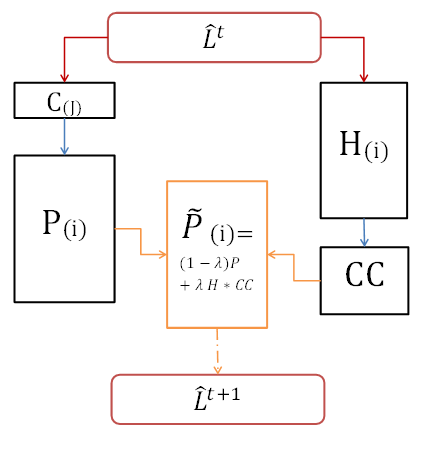
\includegraphics[scale=0.5]{Scheme1.png}} $
		\qquad
		\qquad
		$ \underset{(b)}{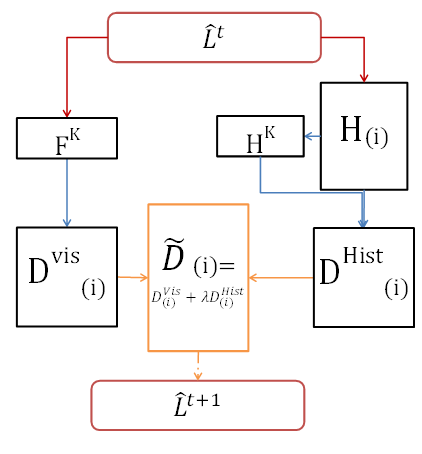
\includegraphics[scale=0.5]{Scheme2.png}} $
		\caption[]{Block diagram (a) Joint Probability method. (b) Mutual distance}
		\label{fig:Scheme}
	\end{center}
\end{figure}

\subsubsection{Hard Thresholding CC}
A simple empirical test can show that natural images contain a sparse Co-Occurrence  matrix, this goes with our assumption that textures (whether smooth or complex) are populated with a low number of different clusters. Thus learning from your environment in label space can be valuable.

We can see this, as a minimization problem:
\begin{equation}
\min\sum_i dist(W_{(i)},C_{\hat L_(i)})+\lambda\lVert CC\rVert_0 \label{eq:minimizer}\\
\end{equation}
minimizing the distance is equivallent to maximaizing the probability\\
in diffrent notation:
\begin{align}
&\min\sum_i \psi_i +\lambda\sum_{i,m}\lVert\phi_{i,m}\rVert_0 \\
&\psi_i=dist(P_{(i)},C_{\hat L_(i)} \nonumber\\
&\phi_{i,m}=CC\nonumber \\
\text{or  } \nonumber\\
&\phi_{i,m}=Pr\{\hat L(i)=J\|\hat L(m)=K\}\;\text{,  s.t m}\in \mathcal{N}(i)\nonumber
\end{align}

i.e. we want small distance between $W_{(i)}$ and $C_{(J)}$, and also minimizing the Co-Occurrence matrix to be sparse such that it will encourage neighborhoods (textures like) containing fewer labels

\subsection{Mutual distance}
Another way of looking at our objective function, is by trying to minimize a mutual distance in both feature spaces, together with finding the best clustering.
\begin{equation}
\min_{\{S_k , F^k,H^k\}} \sum_k \sum_{i\in S_k} dist_v(W_{(i)},F^k)+\lambda dist_H(H_{(i)},H^k)
\end{equation}
such that $ S_k=\{i\in cluster k\} $ and $ F^k,H^k $ are the cluster representative in visual and label histogram space respectively.\\
we will define $ dist_v $- as a simple $ l_2\,norm $, and $ dist_H $-as an EMD (Earth Movers Distance), based on ground distance which is the euclidean distance between $ F^K,F^J $, clusters representatives in visual space (we will see a way to bound this distance in O(n)).\\
%\begin{figure}
%	\begin{center}
%		\caption{mutual distance Scheme}
%		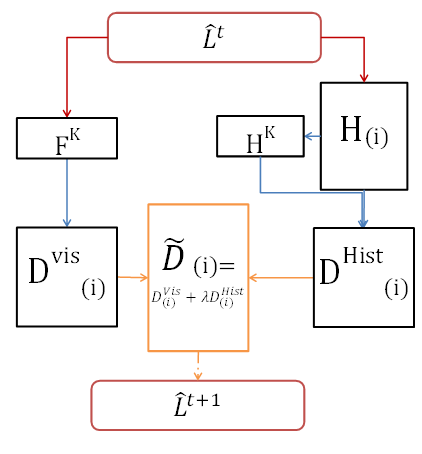
\includegraphics[scale=0.5]{Scheme2.png}
%		\label{fig:mutualdistanceScheme}
%	\end{center}
%\end{figure}

\section{convergence proof}
Only for joint probability:

Both Centers choose and labeling are just like k-means convergence proof, if there is a distance function for histogram space then in the same way we know that we choose the best 

\section{Others Co-Occurrences}

Our basic Co-Occurrence form is show at \eqref{eq:CoOc}, we showed an update rule for each pixel based on passing information from his surrounding.
An other alternative method is calculating the Maximum Likelihood for the center pixel. maximizing The probability of the histogram given a certain label for the center pixel.
\begin{align}
\hat{L}(i)&=\argmax_K \Pr \{H_{(i)}|\hat{L}(i)=K \}\\
&=\sum_{j\in\mathcal{N}(i)}^{} \Pr \{\hat{L}(j)|\hat{L}(i)=K \}\cdot \Pr \{j\}\nonumber
\end{align}
This result a simple correlation distance between the neighborhood histogram $ H_{(i)} $ and the typical histogram for label K $ CC_k $.
As we mentioned before the CC matrix is not symmetric, hence the use of those two method to update $ P_{(i)} $ will result different estimators.

Another problem of the conditional CC is that label with low frequency will tend to disappear after some regularization. The reason is that we prefer to use a low amount of label to describe a texture and adding a low frequent label we drag a high penalty to this.

We can normalize our Co-Occurrence matrix to take into account the frequncy the label.
The first way was showed in \eqref{eq:jointprob} is the joint probability of two label to co occur in the same window.
The second can be thought as 'Mutual Information' variant which tells us how much the two label co occurring is unique.
\begin{equation}
M(K;J)=\dfrac{P(K|J)}{|K|}
\end{equation} 

\end{document}

%\subsection{Co-Occurrence-old ver}
%Co-Occurrence is this space equivalent to center in visual space.
%
%\begin{align}
%&CC_J=\dfrac{1}{|J|} \Sigma_{\hat{L}(i)=J}\frac{H_{(i)}}{W_2^2-1}\\
%&CC=\text{INDICATOR} \cdot H\nonumber\\
%&\text{INDICATOR}[i,J]:=\begin{cases}
%1, &\text{ if }\hat L_(i)=J\nonumber\\
%0, &\text{ else}
%\end{cases}
%\end{align}							
%
%Similar to visual space, we can think of $E_H$ as the probability that $P_{(i)}\in cluster J$ , according to spatial data from labels histogram space.\\
%We can think on message passing from all of $P_i$ neighbors, each neighbor thinks its surrounding should be like his Co-Oc. So $E_H(i)$ is an average of all his neighbors.\\
%Back to our Image I, we introduce the matrix L:\\
%L[i,J]=$\Pr(P_{(i)}\in cluster J)$. Our objective function, $\hat L_{(i)}: (1,..,n)\rightarrow (1,..,K)$ is the maximum likelihood estimator.\\
%$\hat L_{(i)}=  arg\underset {\mathclap {J}}max \, \Pr(P_{(i)}\in cluster J)$.